\scanpage{37}

\figure{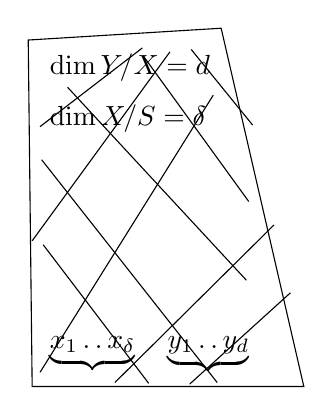
\begin{tikzpicture}[x=1cm,y=1cm]
\draw (0,0)--(-.05,4.4)--(2.4,4.55)--(3.45,0)--cycle;
\node[anchor=west] at (.1,4.05) {$\deleted{\dim Y/X=d}$};
\node[anchor=west] at (.1,3.4) {$\deleted{\dim X/S=\delta}$};
\node[anchor=west] at (.1,.4) {$\deleted{\underbrace{x_1\mathinner{\ldotp\ldotp}x_\delta}\quad\underbrace{y_1\mathinner{\ldotp\ldotp}y_d}}$};
\draw (.1,3.3)--(1.4,4.3) (0,1.85)--(1.75,4.25) (.1,.18)--(2.3,3.7) (1.05,.05)--(3.07,2.05) (2,.03)--(3.28,1.19);
\draw (.14,1.8)--(1.48,.04) (.12,2.88)--(2.35,.05) (.45,3.8)--(2.72,1.35) (1.41,4.2)--(2.75,2.35) (2.02,4.28)--(2.8,3.32);
\end{tikzpicture}}

\uline{\S1} Descente \inserted{d'objet plat} par morphismes quelconques

% slanted
\margin{intervertir ?}

\uline{\S2} Descente d'objet quelconque par morphismes plats.

\uline{\S3} Application \inserted{du \S1} aux morphismes non ramifiés

\uline{\S4} Cas particuliers élémentaires : \unsure{Espaces|Espace} $X/G$; descente galoisienne non ramifiée, le \uline{contre-exemple de Nagata}. Interprétation de la descente plate \uline{finie par quotients} \unsure{groupe|quasi} différentiel. Cas de Cartier.

% slanted
\margin{Le troisième \unsure{alinéa|ordre} du \S1 n'est pas utilisé \unsure{aux|dans les} \S\S1 à 7}

% slanted
\margin{\uline{\unsure{Considérer} descente d'un fibré} \uline{principal} ? \uline{Pas ici le} \uline{lieu}, mais \unsure{renvoyer}}

\uline{\S5} $\underline{\mathrm{Hom}}_S(X,Y)$ et $f_*(X)$ : formalisme général, cas d'existence pour $X$ fini et plat sur $S$. [Est lié à la technique de descente \deleted{\unsure{seulement}} par deux endroits a) Existence de \uline{Hom} si $X\to S$ est géom. injectif -- fini et plat -- b) Relations entre l'existence des $f_*(X)$, $\underline{\mathrm{Hom}}_S(X,Y)$, et les possibilités de descente.] Cas particuliers : $\check{V}(F)$ etc.

% slanted
\margin{propriétés diverses de permanence}

\uline{\S6} Application des schémas \uline{Hom} : la géométrie différentielle les \unsure{$P^i$ envir.|$P^i$ env.|Picard}, Greenberg d'égale caractéristique etc

% slanted
\margin{\uline{ailleurs ?} Ne vient ici que par l'utilisation dans un cas \unsure{bien banal} de l'existence de $f_*$. Pourrait venir \unsure{entièrement|aussi bien} dès le Chap \uline{IV}, mais obligerait d'y développer déjà un \unsure{bout|nº} des \uline{Hom}}

\uline{\S7} Hyper\deleted{\unsure{groupes}}\unsure{schémas|schèmes|thèses} sur $S$. Critère de représentabilité.

[y inclure aussi le critère général d'existence par théorie des modules formels]

\uline{\S8} \unsure{4|A} \deleted{\unsure{Cas particuliers}}\inserted{Théorèmes} \uline{fondamentaux d'existence}

A) Théorie formelle des modules. Extension des \unsure{sections|relations|solutions}.....

\uline{\S9} B) \deleted{\unsure{Hom}} $f_*(X)$ si $X$ est projectif sur $Y$, $Y$ plat et propre sur $S$.

\uline{\S10} C) Picard.

% slanted
\margin{ensemble ?}

[Critères de simplicité, de propreté, de platitude ?]

% archive sheet number: 36
